% architecture_simple.tex — Single-panel simplified architecture diagram
% Compile with: pdflatex architecture_simple.tex
\documentclass[border=5pt]{standalone}
\usepackage[T1]{fontenc}
\usepackage{amssymb}
\usepackage{tikz}
\usetikzlibrary{arrows.meta, positioning, calc, decorations.pathmorphing}

% Colours
\definecolor{cData}{HTML}{C8E6C9}    \definecolor{cDataB}{HTML}{4CAF50}
\definecolor{cFrz}{HTML}{BBDEFB}     \definecolor{cFrzB}{HTML}{1976D2}
\definecolor{cTrn}{HTML}{FFE0B2}     \definecolor{cTrnB}{HTML}{F57C00}
\definecolor{cCch}{HTML}{E1BEE7}     \definecolor{cCchB}{HTML}{8E24AA}
\definecolor{cLoss}{HTML}{FFCDD2}    \definecolor{cLossB}{HTML}{D32F2F}
\definecolor{cOu}{HTML}{F5F5F5}      \definecolor{cOuB}{HTML}{757575}
\definecolor{cBP}{HTML}{C62828}      \definecolor{cG}{HTML}{616161}

\begin{document}
\sffamily
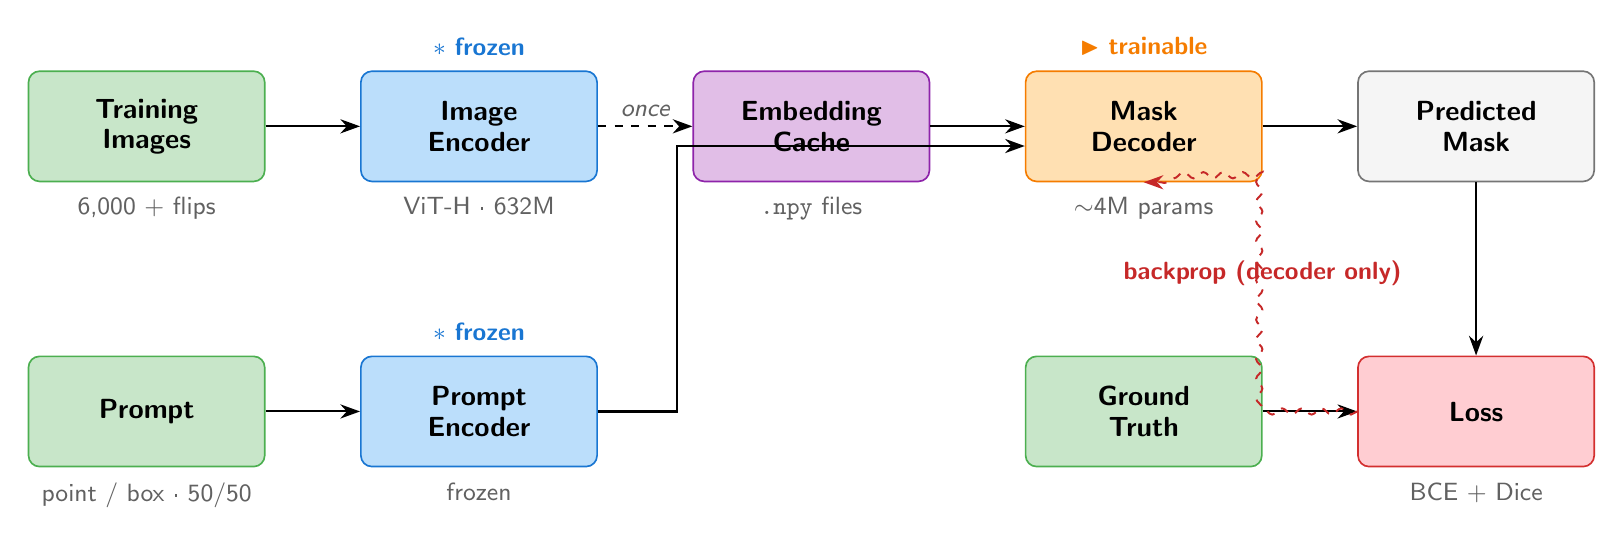
\begin{tikzpicture}[
    nd/.style={rounded corners=4pt, minimum height=14mm, minimum width=30mm,
               align=center, font=\normalsize\sffamily\bfseries, line width=0.6pt},
    ndata/.style ={nd, fill=cData, draw=cDataB},
    nfrz/.style  ={nd, fill=cFrz,  draw=cFrzB},
    ntrn/.style  ={nd, fill=cTrn,  draw=cTrnB},
    ncch/.style  ={nd, fill=cCch,  draw=cCchB},
    nlos/.style  ={nd, fill=cLoss, draw=cLossB},
    nout/.style  ={nd, fill=cOu,   draw=cOuB},
    ar/.style={-{Stealth[length=2.5mm,width=1.8mm]}, line width=0.7pt},
    da/.style={ar, dashed},
    sub/.style={font=\small\sffamily, text=cG, align=center},
    tag/.style={font=\small\sffamily\bfseries, align=center},
]

% === ROW 1: Images → Encoder → Cache → Decoder → Mask ===
\node[ndata] (img) {Training\\[-1pt]Images};
\node[sub, below=2pt of img] {6,000 + flips};

\node[nfrz, right=12mm of img] (enc) {Image\\[-1pt]Encoder};
\node[sub, below=2pt of enc] {ViT-H \textperiodcentered\ 632M};
\node[tag, above=2pt of enc, text=cFrzB] {$\ast$ frozen};

\node[ncch, right=12mm of enc] (cache) {Embedding\\[-1pt]Cache};
\node[sub, below=2pt of cache] {\texttt{.npy} files};

\node[ntrn, right=12mm of cache] (dec) {Mask\\[-1pt]Decoder};
\node[sub, below=2pt of dec] {${\sim}$4M params};
\node[tag, above=2pt of dec, text=cTrnB] {$\blacktriangleright$ trainable};

\node[nout, right=12mm of dec] (pred) {Predicted\\[-1pt]Mask};

% Row 1 arrows
\draw[ar] (img) -- (enc);
\draw[da] (enc) -- node[above, font=\small\sffamily\itshape, text=cG] {once} (cache);
\draw[ar] (cache) -- (dec);
\draw[ar] (dec) -- (pred);

% === ROW 2: Prompt → Prompt Encoder → feeds into Decoder ===
\node[ndata, below=22mm of img] (prm) {Prompt};
\node[sub, below=2pt of prm] {point / box \textperiodcentered\ 50/50};

\node[nfrz, right=12mm of prm] (pe) {Prompt\\[-1pt]Encoder};
\node[sub, below=2pt of pe] {frozen};
\node[tag, above=2pt of pe, text=cFrzB] {$\ast$ frozen};

\draw[ar] (prm) -- (pe);
\draw[ar, line width=0.8pt] (pe.east) -- ++(10mm,0) |- ([yshift=-2.5mm]dec.west);

% === LOSS (below predicted mask) ===
\node[nlos, below=22mm of pred] (loss) {Loss};
\node[sub, below=2pt of loss] {BCE + Dice};

\node[ndata, left=12mm of loss] (gt) {Ground\\[-1pt]Truth};

\draw[ar] (pred) -- (loss);
\draw[ar] (gt) -- (loss);

% === BACKPROP arrow ===
\draw[da, cBP, line width=0.7pt,
      decorate, decoration={snake, amplitude=0.4mm, segment length=2.5mm,
                            post length=1.8mm}]
    (loss.west) -- +(-12mm, 0) |- (dec.south)
    node[pos=0.35, below, font=\small\sffamily\bfseries, text=cBP] {backprop (decoder only)};

\end{tikzpicture}
\end{document}
